\chapter{Matrix Group}
\section{Linear Groups}

\begin{defn}[normal subgroup]
A \textbf{normal subgroup} $N$ of a given group $G$ is a subgroup which left and right cosets $gN$ and $Ng$ are the same: $gN = Ng$, i.e., $$gNg^{-1} = N$$ for every $g\in G.$ We denote it as $N \triangleleft G$.
\end{defn}
\begin{prop}[why normal?] The quotient group $G/N$ (read $G$ mod $N$) is well-defined if and only if $N$ is normal of G.
\end{prop}
\begin{proof}
Whatever we take, the equivalence class must be the same. If $N$ is normal and letting $x\sim \tilde x$, i.e., $x^{-1}\tilde x \in N$, $$\tilde xN \subseteq (xN)N = xN$$ and \textit{vice versa}. If $\bar x = \bar{\tilde x} $ if $x\sim \tilde x$ and $\overline{xy} = \bar x \bar y,$ we have $$gN = (1g)N = NgN = hNgN = (hg)N$$ for every $h\in N$, hence $N = g^{-1} hgN$ so that $N$ is normal: letting $n = g^{-1}hg\tilde{n}$, we have $g^{-1}hg=n\tilde{n}^{-1}\in N$ for every $h\in N$ whence $g^{-1}Ng \subseteq N.$
\end{proof}
\begin{defn}[general linear group and special linear group] The \textbf{general linear group} of a given vector space $V$ is a (multiplicative) group of automorphism on $V$; that is, $\operatorname{GL}(V) = \mathfrak L(V,V)^\times.$ And the \textbf{special linear group} of $V$ is the subgroup of $\operatorname{GL}(V)$ which is consisted by linear transformations whose determinant are all 1.

We denote $\operatorname{GL}(n, F) = \operatorname{GL}(F^n),$ and $\operatorname{SL}(n, F) = \operatorname{SL}(F^n).$
\end{defn}
\begin{theorem}[first isomorphism theorem]
For any homomorphism $\varphi:~G\to H$ for two groups $G$ and $H$, $$G/\ker \varphi \approx \operatorname{im} \varphi.$$
\end{theorem}
\begin{proof}
\hfill
\begin{center}
\leavevmode
\xy
\xymatrix {
G \ar@{->}[rr]^{\varphi} \ar@{->}[dr] &&\operatorname{im}\varphi\\ & G/\operatorname{ker}\varphi \ar@{->}[ur]_{\approx} &\\
}
\endxy
\end{center}
\end{proof}
\begin{prop}[GL and SL] $$\operatorname{GL}(V)/\operatorname{SL}(V) \approx F^\times.$$
\end{prop}

\begin{defn}[center] The \textbf{center} $Z(G)$ of a group $G$ is the subgroup of elements which satisfy the `commutative law', i.e., $$Z(G) = \{z\in G: \quad zg = gz \textrm{ for every }g\in G\}.$$ $Z$ for \textit{zentrum}, which means `center' in German.
\end{defn}
\begin{prop}[normality of the center]
$$Z(G)\triangleleft G.$$
\end{prop}
\begin{proof}
Trivially, $$gZ(G) = \{gz:~z\in Z(G)\} = \{zg:~z \in Z(G)\} = Z(G)g.$$
\end{proof}
\begin{ex}
What are the centers of (a) $\operatorname{GL}(n, F)$ and (b) $\operatorname{SL}(n, F)$?

Answer: (a) $0\ne cI$'s, (b) $\alpha I$'s where $\alpha^n = 1.$
\end{ex}
\begin{proof}
(a) is just all. Let $AZ = ZA$ for all invertible $A.$ Then, especially, for all \textit{elementary matrices}, $EZ = ZE.$ Note that multiplying $E$ left is the same with elementary \textit{row} operating, while multiplying right is for elementary \textit{column} operating. (Especially, for $E_{i + cj}$'s.) Hence we obtain that $Z$ is diagonal. Instead a more detailed explanation, we see an example: $$
\begin{pmatrix}
1 & 3 \\
0 & 1
\end{pmatrix}
\begin{pmatrix}
a & *_1 \\
*_2 & b
\end{pmatrix}
=
\begin{pmatrix}
a + 3*_2 & *_1 + 3b \\
*_2 & b
\end{pmatrix},$$
$$\begin{pmatrix}
a & *_1 \\
*_2 & b
\end{pmatrix}
\begin{pmatrix}
1 & 3 \\
0 & 1
\end{pmatrix}
=
\begin{pmatrix}
a  & *_1 + 3a \\
*_2 & b + 3*_2
\end{pmatrix},$$
hence $*_1$ and $*_2$ are zero. Similar details says that $Z$ must be diagonal, for bigger matrices.

Now, the proof is done: since $E_{i\leftrightarrow j}$ is an elementary matrix, $Z_{ii} = Z_{jj}$, for every $i$ and $j$ pair. Therefore $Z$ is a `nonzero'(since $Z$ is invertible!) multiple of $I.$

Not so surprisingly, the proof works on any \textit{ring} with 1; if we modify `nonzero' to `invertible', that is, $c\in R^{\times}.$
\end{proof}
\begin{add}[divide by center?] Dividing by center means to ignore the difference due to the elements of $Z.$ Since $$Z(G) = \{z\in G:\quad z = gzg^{-1}\textrm{ for every }g\in G\},$$ we have some `morphisms' $\varphi_g:~a \mapsto b = gzg^{-1}$ and \textit{their group} $$\operatorname{Inn}(G) = \{ \varphi_g:\quad g \in G\}.$$ We call this group the \textbf{inner automorphism group} of $G$.

We want to show that $G/Z(G) \approx \operatorname{Inn}(G).$ The idea is easy: use the homomorphism $\varphi_\bullet$ above: $$\varphi_\bullet:\quad G \to \operatorname{Inn}(G).$$ The kernel of this homomorphism is just the center of $G$, since the (multiplicational) identity of $\operatorname{Inn}(G)$ is the identity function $\operatorname{id}_G$ and, from $$\varphi_z = z\bullet z^{-1} = \operatorname{id}_G, \qquad \forall g\in G,$$i.e., $$\varphi_z (g) = zgz^{-1} = g, \qquad \forall g\in G,$$ we get $zg = gz$ whence $z \in Z(G).$ Therefore $\ker (\varphi_\bullet) = Z(G)$, and by the first isomorphism theorem, we obtain $$G/Z(G) \approx \operatorname{Inn}(G).$$
\end{add}

\begin{defn}[PGL and PSL]
The \textbf{projective general linear group} is defined by $$\operatorname{PGL}(V) = \operatorname{GL}(V)/Z(\operatorname{GL}(V)).$$
The \textbf{projective special linear group} is defined by $$\operatorname{PSL}(V) = \operatorname{SL}(V)/Z(\operatorname{SL}(V)).$$
\end{defn}

Projective geometry is difficult...

\section{Orthogonal group}
\begin{defn}[orthogonal transformation]
For an \textit{inner product space} $(V,~\langle \bullet , \bullet \rangle)$ (or even just a quadratic space with non-degenerate symmetric bilinear form), an \textbf{orthogonal transformation} of $V$ is an invertible linear transformation which preserves the given inner product, that is, such $A\in \operatorname{GL}(V)$: $$\langle v, ~w \rangle = \langle Av,~ Aw \rangle.$$ The group of such transformations is called the \textbf{orthogonal group} $\operatorname{O}(V)$ of $V$, and also denote $\operatorname{O}(n, F) = \operatorname{O}(F^n)$ and $\mathrm O(n) = \mathrm O(n, \mathbb R)$. $F^n$ is considered with \textit{dot product.}

Similarly, $\operatorname{SO}(V) = \{T\in \operatorname{O}(V):~ \operatorname{det}T = 1\}$, and analogous definitions for $\operatorname{SO}(n,F)$ and $\operatorname{SO}(n).$ Obviously, it is called the \textbf{special orthogonal group} of $V$.
\end{defn}
\begin{defn}[unitary group]
If we give a \textit{hermitian form} $(V, ~ \langle \bullet, \bullet \rangle )$ rather than an inner product, where the given field is `trivially' the field $\mathbb C$ of complex number, we define analogously \textbf{unitary group} $\operatorname{U}(n)$ as we defined the orthogonal group:$$\langle v, ~w \rangle = \langle Av,~ Aw \rangle, \qquad A \in \operatorname{GL}(n,~\mathbb C).$$ We \textit{already know} what is $\operatorname{SU}(n)$ and how to call it \textsf{:D}.
\end{defn}

\begin{prop}
\hfill
\begin{itemize}
    \item $\operatorname{SO}(V) \triangleleft\operatorname{O}(V) \triangleleft \operatorname{GL}(V);$
    \item $\operatorname{SO}(V) \triangleleft\operatorname{SL}(V) \triangleleft \operatorname{GL}(V);$
    \item $\operatorname{O}(n, F) = \{ A\in \mathfrak M_{n,n}(F)^\times:~ A^{-1}=A^\mathsf T\},$ if the inner product is a standard one, so-called \textit{dot product}. (\textit{Canonically isomorphic!})
\end{itemize}
Also the followings hold: for $\operatorname{O}(n, F)$,  every element is a matrix with pairwise orthonormal columns (or rows).
\end{prop}
Good, well, why it is called `orthogonal'? It is because these preserves the `angle' of two vectors, especially the \textit{orthogonality}. Then, \textit{what} is orthogonal? Which matrices are orthogonal?
\begin{prop}
\hfill

In $\mathbb R^2$, $\operatorname{O}(2)$ consists of rotations and reflections. And the group of rotations is just $\operatorname{SO}(2).$
\begin{proof}From
$$A=\begin{pmatrix}a&b\\c&d\end{pmatrix}, \qquad AA^\mathsf T = \begin{pmatrix}a&b\\c&d\end{pmatrix}\begin{pmatrix}a&c\\b&d\end{pmatrix} = \begin{pmatrix}a^2+b^2&ac+bd\\ac+bd&c^2+d^2\end{pmatrix} = I,$$
we obtain $a^2 + b^2 = 1 = c^2 + d^2$ and $ac+bd = 0$. Solutions for the first equality are just sines and cosines, namely: $$a = \cos x, ~~b = \sin x, \quad c = \cos y,~~d = \sin y.$$ (Orders of sine and cosine do not have to consider; since there is an inversion $\theta~\mapsto~\frac \pi 2 - \theta$.) Evaluating to another equality, $$\cos x \cos y + \sin x \sin y = \cos(y-x) = 0,\qquad y-x = \frac{2k-1}{2}\pi.$$ Hence $y = x + \frac{2k-1}{2}\pi.$ Substituting it, we get $$c = - \sin x \sin \left(\frac{2k-1}{2}\pi\right) = \mp \sin x,\qquad d = \cos x \sin \left(\frac{2k-1}{2}\pi\right) = \pm \cos x.$$ Due to a \textit{custom} in math and other sciences, we use $\theta = -x$ and finally get $$A=\begin{pmatrix}\cos \theta &-\sin \theta \\ \pm \sin \theta & \pm \cos \theta \end{pmatrix}.$$

If the signa of second row are pluses, $$A_+ = \begin{pmatrix}\cos \theta &-\sin \theta \\\sin \theta & \cos \theta \end{pmatrix} = R_\theta,$$ where $R_\theta$ is the \textbf{rotation matrix} of angle $\theta$. Since $ \operatorname{det}R_\theta = 1$, $R_\theta \in \operatorname{SO}(2).$

If the signa of second row are minuses, $$A_- = \begin{pmatrix}\cos \theta &-\sin \theta \\-\sin \theta & -\cos \theta \end{pmatrix}  = \begin{pmatrix}1&0\\0&-1\end{pmatrix} \begin{pmatrix}\cos \theta &-\sin \theta \\\sin \theta & \cos \theta \end{pmatrix} =\begin{pmatrix}1&0\\0&-1\end{pmatrix} R_\theta = S_{-\theta/2},$$ where $S_\varphi$ is a \textbf{reflection matrix} w.r.t. a line $\theta = \varphi$ in polar coordinate system. (Draw it $\sim \!.$) Note that $\operatorname{det}S_\varphi = -1$.
\end{proof}
\end{prop}

How about 3-dimensional space? We consider a rotation on a line, the \textit{axis}. For example, there are `basic' three rotations: $$\displaystyle {\begin{alignedat}{1}R_{x}(\theta )&={\begin{pmatrix}1&0&0\\0&\cos \theta &-\sin \theta \\[3pt]0&\sin \theta &\cos \theta \\[3pt]\end{pmatrix},}\\[6pt]R_{y}(\theta )&={\begin{pmatrix}\cos \theta &0&\sin \theta \\[3pt]0&1&0\\[3pt]-\sin \theta &0&\cos \theta \\\end{pmatrix},}\\[6pt]R_{z}(\theta )&={\begin{pmatrix}\cos \theta &-\sin \theta &0\\[3pt]\sin \theta &\cos \theta &0\\[3pt]0&0&1\\\end{pmatrix}.}\end{alignedat}}$$ Surprisingly, they are almost \textit{all}, i.e., the following holds. (Details are omitted.)

\begin{theorem}[decomposition of rotation]
For every `rotation' $R\in\operatorname{SO}(3)$,
$$R=R_{z}(\alpha )\,R_{y}(\beta )\,R_{x}(\gamma )\,$$
 where \textit{Tait-Bryan angles} of $R$ are $\alpha$, $\beta$, $\gamma$, about axes $z$, $y$, $x$ respectively.
\end{theorem}

Following our knowledge, there efinition for \textit{arbitrary rotation} is quite obvious, and only acceptable:

\begin{defn}[rotation] \textbf{Rotation} is an element of SO.\end{defn}

We must figure out the following definitions.
\begin{defn}[PGO, PSO, PGU, PSU]Projective (general) orthogonal group $\operatorname{PGO}(V)$ and projective special orthogonal group $\operatorname{PSO}(V).$ Similarly for U's...
\end{defn}
\begin{ex}
Calculate them! What is $Z(\operatorname{O}(V))$ and $Z(\operatorname{SO}(V))$?
\end{ex}
\begin{proof}
Same with \textbf{Example 1.1.} A difference is that $\det Z = \pm 1$ in $\operatorname{O}(V).$ Another one is for $\operatorname{SO}$: for odd-dimensional $V$, $Z(\operatorname{SO}(V))=\{I\}$ (a trivial group) since $\operatorname{det}\pm I = \pm 1$; while $Z(\operatorname{SO}(V))=\{\pm I\}$ for even-dimensional $V$ since $\operatorname{det}\pm I = 1.$
\end{proof}
\begin{coro}
\emph{PSO $\approx$ SO} for odd-dimensional vector space $V$.
\end{coro}
\begin{prop}
$$\operatorname{PSU}(2)\approx \operatorname{SO}(3), \qquad \operatorname{SU}(2) \dhxrightarrow{\text{double}} \operatorname{SO}(3),$$ where $\dhxrightarrow{\text{double}}$ means that there is a double covering.
\end{prop}

``The shortest path between two truths in the real domain passes through the complex domain.'' ---Jacques Hadamard.

\begin{proof}
$Z(\operatorname{SU}(2)) = \{\pm I\}$? Trivial. Then it suffices to show that $\operatorname{PSU}(2)\approx \operatorname{SO}(3)$. A transformation $A$ of $\operatorname{PSU}(2)$ satisfies \textsf{(U)} $AA^\dagger = I$ by the definition. Use same method as \textbf{Proposition 1.5.}: let $$A=\begin{pmatrix}a&b\\c&d\end{pmatrix},$$ then $$AA^\dagger = \begin{pmatrix}a&b\\c&d\end{pmatrix}\begin{pmatrix}\bar a&\bar c\\\bar b&\bar d\end{pmatrix} = \begin{pmatrix}a\bar a+b\bar b&a\bar c+b\bar d\\\bar a c+\bar b d&c\bar c + d\bar d\end{pmatrix}=I$$ whence $$|a|^2 + |b|^2 = 1 = |c|^2 + |d|^2, \qquad a\bar c + b\bar d = 0.$$ The first equality gives us $$a = e^{i\varphi_1}\cos x,~~b = e^{i\varphi_2}\sin x,~~c = e^{i\varphi_3}\cos y,~~d = e^{i\varphi_4}\sin y,$$ and the second equality gives $$\cos x \cos y + e^{i(-\varphi_1+\varphi_2+\varphi_3-\varphi_4)}\sin x \sin y = 0,$$ since $\overline{e^{i\theta}} = e^{-i\theta}$ for real $\theta$. If $-\varphi_1+\varphi_2+\varphi_3-\varphi_4 \ne 0,$ the equality must not hold unless $b=d=0$, which leads to a contradiction. Also, since \textsf{(S)} $\operatorname{det}A = 1$, $$ad-bc = e^{i(\varphi_1 + \varphi_4)}(\cos x \sin y - \sin x \cos y) = e^{i(\varphi_1 + \varphi_4)} \sin(y-x) = 1$$ whence $\varphi_1 + \varphi_4 =\varphi_2 + \varphi_3 = k\pi$ and $y-x = \frac{2k-1}{2} \pi.$ Therefore $$A = \begin{pmatrix}e^{i\varphi_1}\cos x&e^{i\varphi_2}\sin x \\ \mp e^{- i\varphi_2}\sin x&\pm e^{-i\varphi_1}\cos x \end{pmatrix}.$$ Finally, \textsf{(P)} ignore one signum of them, then we have $$A = \begin{pmatrix}e^{i\varphi_1}\cos \theta & - e^{i\varphi_2}\sin \theta \\  e^{- i\varphi_2}\sin \theta& e^{-i\varphi_1}\cos \theta \end{pmatrix}.$$ Hence, for example, there is an `isomorphism' $$\begin{pmatrix}e^{i\varphi_1}\cos \theta & - e^{i\varphi_2}\sin \theta \\  e^{- i\varphi_2}\sin \theta& e^{-i\varphi_1}\cos \theta \end{pmatrix} \leftrightarrow (\theta, \varphi_1, \varphi_2) \leftrightarrow R_z(\theta)R_y(\varphi_1)R_x(\varphi_2),$$ since $R_\bullet (\alpha + \beta) = R_\bullet (\alpha)R_\bullet (\beta).$ Therefore $\operatorname{PSU}(2)\approx \operatorname{SO}(3).$
\end{proof}
\section{SO(1,1)}
\begin{defn}[indefinite orthogonal group] Consider the Euclidean space only, i.e.,   $F=\mathbb R$.
The \textbf{indefinite orthogonal group} $\operatorname{O}(p, q)$ is something like O, but the inner product is not provided while the following bilinear form is given: $$\langle v, w\rangle = v^\mathsf T \operatorname{diag}(\underbrace{1, \cdots, 1}_{p}, \underbrace{-1, \cdots, -1}_{q}) w,$$
 for $(p+q)$-dimensional vectors $v$ and $w$. For instance, $\operatorname{O}(n) = \operatorname{O}(n,0) = \operatorname{O}(0,n).$
And SO$(p,q)$ is ...
\end{defn}
We are interested in O(1,1) and O(1,3) in particular.
\begin{prop}
$\operatorname{SO}(1,1)$ can be represented by a hyperbolae $x^2 - y^2 = 1$, hence 2 connected curves. $\operatorname{SO}^+$ is the `connected' component of this group which contains the identity $I$, $$\operatorname{SO}^+ = \left\{ \begin{pmatrix}\cosh \theta & \sinh \theta \\ \sinh \theta & \cosh \theta\end{pmatrix}:~~ \theta\in\mathbb R \right\}.$$ In fact, we call the connected component of a given `topological' group that contains the identity element the \textbf{identity component} of given group.
\end{prop}
\begin{center}

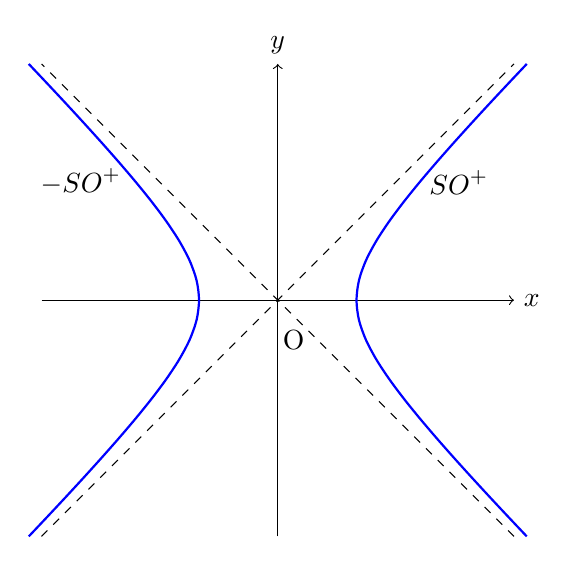
\begin{tikzpicture}
\draw[->] (-3,0) -- (3,0) node[right] {$x$};
\draw[->] (0,-3) -- (0,3) node[above] {$y$};
\draw[dashed] (-3,-3) -- (3,3);
\draw[dashed] (3,-3) -- (-3,3);
\draw[scale=1,domain=-3:3,smooth,variable=\y,blue,thick] plot ({(\y*\y + 1)^(1/2)},{\y});
\node at (2.3,1.5) {$\operatorname{SO}^{+}$};
\draw[scale=1,domain=-3:3,smooth,variable=\y,blue,thick] plot ({-(\y*\y + 1)^(1/2)},{\y});
\node at (-2.5,1.5) {$-\operatorname{SO}^{+}$};
\node at (0.2,-0.5) {O};
\end{tikzpicture}
\end{center}
\begin{proof}
Completely same process. Note that if $A\in\operatorname{SO}(1,1)$, $$v^\mathsf T \begin{pmatrix}1&0\\0&-1\end{pmatrix}w = \langle v,w\rangle = \langle Av,Aw\rangle =v^\mathsf T A^\mathsf T \begin{pmatrix}1&0\\0&-1\end{pmatrix}Aw,$$ hence $$\begin{pmatrix}1&0\\0&-1\end{pmatrix} = A^\mathsf T \begin{pmatrix}1&0\\0&-1\end{pmatrix} A.$$ Then we have $$\operatorname{SO}(1,1) = \left\{ \pm \begin{pmatrix}\cosh \theta & \sinh \theta \\ \sinh \theta & \cosh \theta\end{pmatrix}:~~ \theta\in\mathbb R \right\}.$$ We \textit{can(?)} represent it as a parametrized hyperbola: $$\pm \begin{pmatrix}\cosh \theta & \sinh \theta \\ \sinh \theta & \cosh \theta\end{pmatrix} \longleftrightarrow \pm\begin{pmatrix}\cosh \theta\\ \sinh \theta\end{pmatrix},$$ then $\operatorname{SO}^+$ and $-\operatorname{SO}^+$ are connected components of $\operatorname{SO}(1,1).$
\end{proof}
What does `connected' means? Detail definition is in \textit{topology}: it cannot separated by some open sets.

We will stop our work here about groups for the time being. If we learn \textit{topology} or \textit{Lie group theory}, it will continue...
